\documentclass[12pt,french]{thesis}
\usepackage[french]{babel}
%\usepackage{amsmath}
\usepackage{tabularx}
%\usepackage[latin1]{inputenc}
\usepackage{ifpdf}
\usepackage{ae}
\usepackage[T1]{fontenc}
\usepackage[final]{pdfpages}
\usepackage{tikz}
\usepackage{verbatim}
\usetikzlibrary{arrows,shapes}
\usepackage[utf8]{inputenc}
\usepackage{changepage} 

%\usepackage{algorithm}
%\usepackage{algorithmic}
%\usepackage{vector}
\usepackage{graphicx,natbib,amssymb,lineno}
%\usepackage{latex8}
\usepackage{color}
\usepackage{subfigure}
\providecommand{\keywords}[1]{\textbf{\textit{Mots clés---}} #1}
\def \cind {\,\bot\hspace{-.50em}\bot\,}
\def \un {\hbox{\rm 1\hskip -2.4pt l}}

\renewcommand{\baselinestretch}{1.5}

\captionheaderfont{\sl\bfseries}
\captionbodyfont{\sl}
\renewcommand{\tableshortname}{Table}
\renewcommand{\figureshortname}{Figure}
\chapapp{\chaptername}

\newcommand{\so}{\mbox{so}}

\newtheorem{theorem}{Théorème}
\newtheorem{definition}{Définition}
\newtheorem{lemma}[theorem]{Lemme}
\newtheorem{examp}{Exemple}
\newtheorem{corol}[theorem]{Corollaire}

\textheight=600pt
\textwidth=450pt
\marginparwidth=1pt
\topmargin=10pt
\oddsidemargin=1pt
\marginparsep=1pt

\newcommand{\reportTitle} {%
  %\textsc{Graduation Project}
  \textsc{Projet de Fin d'études}
}

\newcommand{\reportAuthor} {%
  FirstName \textsc{LastName}%
}

\newcommand{\reportSubject} {%
  Le titre du rapport
}

\newcommand{\dateSoutenance} {%
  12/06/2024%
}

%\newcommand{\studyDepartment} {%
%  Entreprise d'accueil
%}

\newcommand{\ESAM} {\textbf{E}cole \textbf{S}upérieure d'\textbf{A}griculture de \textbf{M}ograne
}

%\newcommand{\codePFE} {% Reference
%  Code PFE%
%}

\newcommand{\anneeuniv}{
2023-2024}

\usepackage{titlesec}
\titleformat{\chapter}[display]
  {\centering\normalfont\huge\bfseries}{\chaptertitlename\ \thechapter}{14pt}{\Huge}

\begin{document}
% -----------------------------
% PAGE DE GARDE
% -----------------------------

\frontmatter
\title{\vspace{-5cm}

\begin{adjustwidth}{-1cm}{-1cm}
\begin{center}
    \begin{tabular}{p{4cm}p{8cm}p{5.5cm}}
    \centering
\includegraphics[width=0.75\linewidth]{universite-carthage.PNG} \\ 
    \scriptsize \textbf{U}niversité de \textbf{C}arthage& 
    \centering
\includegraphics[width=0.55\linewidth]{embleme.jpg} \\ \scriptsize\textbf{\textbf{République Tunisienne}}\\ \scriptsize Ministère de l'Enseignement Supérieur et de la Recherche Scientifique \& Ministère de l’Agriculture, des Ressources Hydrauliques et de la Pêche & 
    \centering
\includegraphics[width=0.45\linewidth]{ModelePFE_latex ESAM/IRESALOGO.png}\\ \scriptsize Institution de recherche agricole et d'enseignement supérieur \\
    \end{tabular}
\end{center}
\end{adjustwidth}


\begin{center}
    \begin{tabular}{p{8cm}}
    \centering
    
\includegraphics[width=0.35\linewidth]{ModelePFE_latex ESAM/ESAMLOGO.png}\\
    \footnotesize \textbf{Ecole Supérieure d'Agriculture de Mograne}\\
    \end{tabular}
\end{center} 

\begin{center}\small \textbf{\textit{Rapport de Projet de Fin d'Etudes présenté pour l'obtention du}} \end{center}
\begin{center} \normalsize Diplôme National d'Ingénieur en  ....... 
\end{center}

\vspace{-2cm}}


\author{
\large \reportAuthor
\vspace{-2cm}}
\date{\begin{center}
\rule{0.5\textwidth}{.4pt} \\
 \Large \reportSubject \\
\rule{0.5\textwidth}{.4pt}\\
\normalsize Soutenu le~\dateSoutenance~ devant le Jury composé de :\end{center}
\vspace{-1cm}}

\institution{\begin{center}
\begin{itemize}
  \item  Nom et prénom du  member 1,  Grade, Affiliation (Président)
  \item  Nom et prénom du  member 2,  Grade, Affiliation (Rapporteur)
  \item  Nom et prénom du  member 3,  Grade, Affiliation (Encadrant entreprise)
  \item  Nom et prénom du  member 4,  Grade, Affiliation (Encadrant universitaire)
  \end{itemize}
%\textbf{\textit{Stage de Fin d'Études effectué à}}\\
\end{center}
%\begin{minipage}{7cm}\begin{center}\small \textbf{\studyDepartment} \end{center}\end{minipage}  \begin{minipage}{7cm}\begin{center}\includegraphics[width=0.35\linewidth]{ModelePFE_latex ESAM/logo.jpg} \end{center}\end{minipage}
%\vspace{0.1cm}
\begin{center}\small Année universitaire \anneeuniv \end{center}
}

%\dedication{\begin{flushright}\textit{\small{A mes parents, Sameh, Aichoucha et Yassine}}\end{flushright}}
%\uppertitleback{ENIT- Ut\'e de Tunis El Manar}
%\middletitleback{Publication Data:\\
%\tt F. Phidias Fanstord\\
%Fighting Fire with Fire\\
%Festooning French Phrases\\
%Fanstord: Fanstord University Press\\
%ISBN 0-4850}}
%\lowertitleback{Copyright $\copyright$ 1993 Phoney-Baloney}

\dedication{\begin{flushright}\textit{\small{Une d\'edicace \`a ....}}\end{flushright}}



\maketitle

\chapter*{\textit{Remerciements}}
 \textit{
Je souhaite tout d'abord exprimer mes plus vifs et sinc\`eres remerciements }

\begin{abstract}

Un résumé, plus communément appelé "<abstract"> sous sa dénomination anglophone, est un court texte (rarement plus d'une demi-page) qui permet d'introduire le sujet. Il s'agit d'une courte synthèse du travail, un condensé, qui va brièvement annoncer :

*Le contexte du travail : pourquoi s'intéresser à ce sujet ? Qu'est-ce qui motive ce travail ?\\
*La problématique : quel est le problème, la question à laquelle le chercheur essaie de répondre ?\\
*Quelques explications sur l'approche, ou la méthode, employée : comment réussir à résoudre le problème, mais sans rentrer dans les détails.\\
*Les principaux résultats : est-ce que le travail permet de répondre à la question ? Quels sont les résultats marquants qui ont été mis en évidence ?\\
*La conclusion : quelles sont les implications de la réponse qui a été trouvée ? Vers quelle ouverture cela peut-il mener ?

250 mots MAXIMUM. \\

\keywords{insérez quelques mots clés}
\end{abstract}

\tableofcontents

\listoffigures

\listoftables


%\chapter{Preface}

\mainmatter




%\tableofcontents
\chapter*{Introduction}
\addcontentsline{toc}{chapter}{Introduction} 
\chapter{Chapitre 1}

D'après les livres \cite{schaeffer99}, \cite{jenkins2004}, \cite{caillois1}.

Voici une formule de math dans la ligne $x^2=\log(x)$ et une autre au milieu
$$x^2=\displaystyle\frac{2}{3}$$
et
aussi on peut citer l'\'equation (\ref{eq1})
\begin{equation}
x^2=\displaystyle\frac{2}{3} \label{eq1}
\end{equation}
\section{Paragraphe 1}

Le graphique de la figure \ref{fig1}

\begin{figure}[h]
\centering
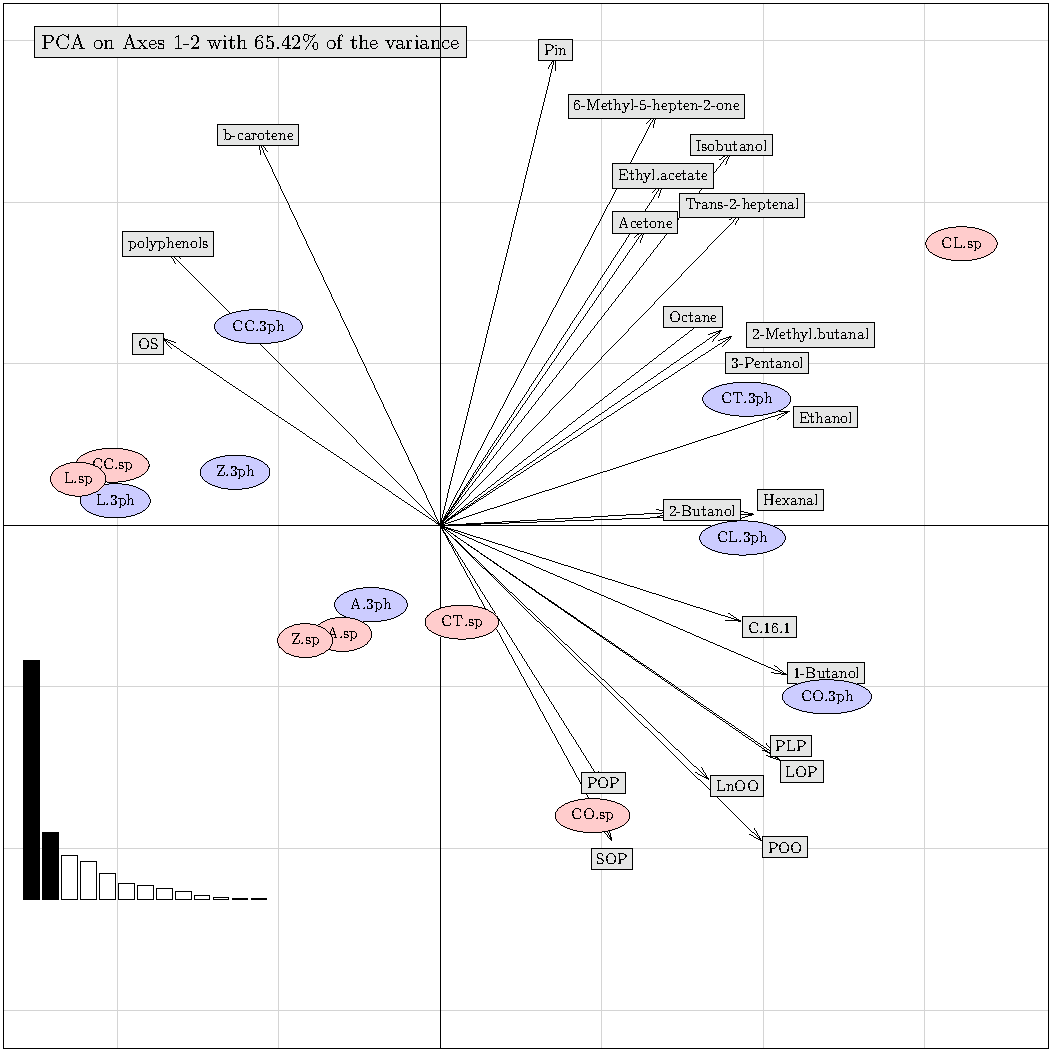
\includegraphics[scale=.5]{acp1}
\caption{Mon graphe \label{fig1}}
\end{figure}

\begin{table}[]
    \centering
    \begin{tabular}{|c||c|c|c|c|}
    \hline
        Variétés & Ph & Poids& Taille& X \\ \hline
        Chemlali & 1.4 & ... & ... &... \\ \hline
        ... & ... & ... &...  &... \\ \hline
    \end{tabular}
    \caption{Statistique descriptive}
    \label{tab:my_label}
\end{table}




\bibliographystyle{abbrvnat}
 \bibliography{Biblio}


\end{document}
